%%%%%%%%%%%%%%%%%%%%%%%%%%%%%%%%%%%%%%%%%
% Beamer Presentation
% LaTeX Template
% Version 1.0 (10/11/12)
%
% This template has been downloaded from:
% http://www.LaTeXTemplates.com
%
% License:
% CC BY-NC-SA 3.0 (http://creativecommons.org/licenses/by-nc-sa/3.0/)
%
%%%%%%%%%%%%%%%%%%%%%%%%%%%%%%%%%%%%%%%%%

% ----------------------------------------------------------------------------------------
% PACKAGES AND THEMES
% ----------------------------------------------------------------------------------------

\documentclass{beamer}

\mode<presentation> {

  % The Beamer class comes with a number of default slide themes
  % which change the colors and layouts of slides. Below this is a list
  % of all the themes, uncomment each in turn to see what they look like.

  % \usetheme{default}
  % \usetheme{AnnArbor}
  % \usetheme{Antibes}
  % \usetheme{Bergen}
  % \usetheme{Berkeley}
  % \usetheme{Berlin}
  % \usetheme{Boadilla}
  % \usetheme{CambridgeUS}
  % \usetheme{Copenhagen}
  % \usetheme{Darmstadt}
  % \usetheme{Dresden}
  % \usetheme{Frankfurt}
  % \usetheme{Goettingen}
  % \usetheme{Hannover}
  % \usetheme{Ilmenau}
  % \usetheme{JuanLesPins}
  % \usetheme{Luebeck}
  \usetheme{Madrid}
  % \usetheme{Malmoe}
  % \usetheme{Marburg}
  % \usetheme{Montpellier}
  % \usetheme{PaloAlto}
  % \usetheme{Pittsburgh}
  % \usetheme{Rochester}
  % \usetheme{Singapore}
  % \usetheme{Szeged}
  % \usetheme{Warsaw}

  % As well as themes, the Beamer class has a number of color themes
  % for any slide theme. Uncomment each of these in turn to see how it
  % changes the colors of your current slide theme.

  % \usecolortheme{albatross}
  \usecolortheme{beaver}
  % \usecolortheme{beetle}
  % \usecolortheme{crane}
  % \usecolortheme{dolphin}
  % \usecolortheme{dove}
  % \usecolortheme{fly}
  % \usecolortheme{lily}
  % \usecolortheme{orchid}
  % \usecolortheme{rose}
  % \usecolortheme{seagull}
  % \usecolortheme{seahorse}
  % \usecolortheme{whale}
  % \usecolortheme{wolverine}

  % \setbeamertemplate{footline} % To remove the footer line in all slides uncomment this line
  % \setbeamertemplate{footline}[page number] % To replace the footer line in all slides with a simple slide count uncomment this line

  % \setbeamertemplate{navigation symbols}{} % To remove the navigation symbols from the bottom of all slides uncomment this line
}

\usepackage{graphicx} % Allows including images
\usepackage{booktabs} % Allows the use of \toprule, \midrule and \bottomrule in tables
% draw shit
\usepackage{tikz}
\usetikzlibrary{fit,arrows,calc,positioning}

\graphicspath{{imgs/}}

% ----------------------------------------------------------------------------------------
% TITLE PAGE
% ----------------------------------------------------------------------------------------

\title[9/25]{SIGAI General Meeting -- 9/25} % The short title appears at the bottom of every slide, the full title is only on the title page

\author{SIGAI} % Your name
\institute[http://sigai.ml] % Your institution as it will appear on the bottom of every slide, may be shorthand to save space
{
  \textit{http://sigai.ml} % Your email address
}
\date{\today} % Date, can be changed to a custom date

\begin{document}

\begin{frame}
  \titlepage % Print the title page as the first slide
\end{frame}

\begin{frame}
  \frametitle{Overview} % Table of contents slide, comment this block out to remove it
  \tableofcontents % Throughout your presentation, if you choose to use \section{} and \subsection{} commands, these will automatically be printed on this slide as an overview of your presentation
\end{frame}

\section{General Annoucements}
\begin{frame}
  \frametitle{General Annoucements}
  \begin{itemize}
  \item ACM Exec Annoucements
  \item SIGAI This Week
    \begin{itemize}
    \item Tensorflow Workshop happened 9/25
    \end{itemize}
  \end{itemize}
\end{frame}

\section{Survey Results}
\begin{frame}
  \begin{center}
    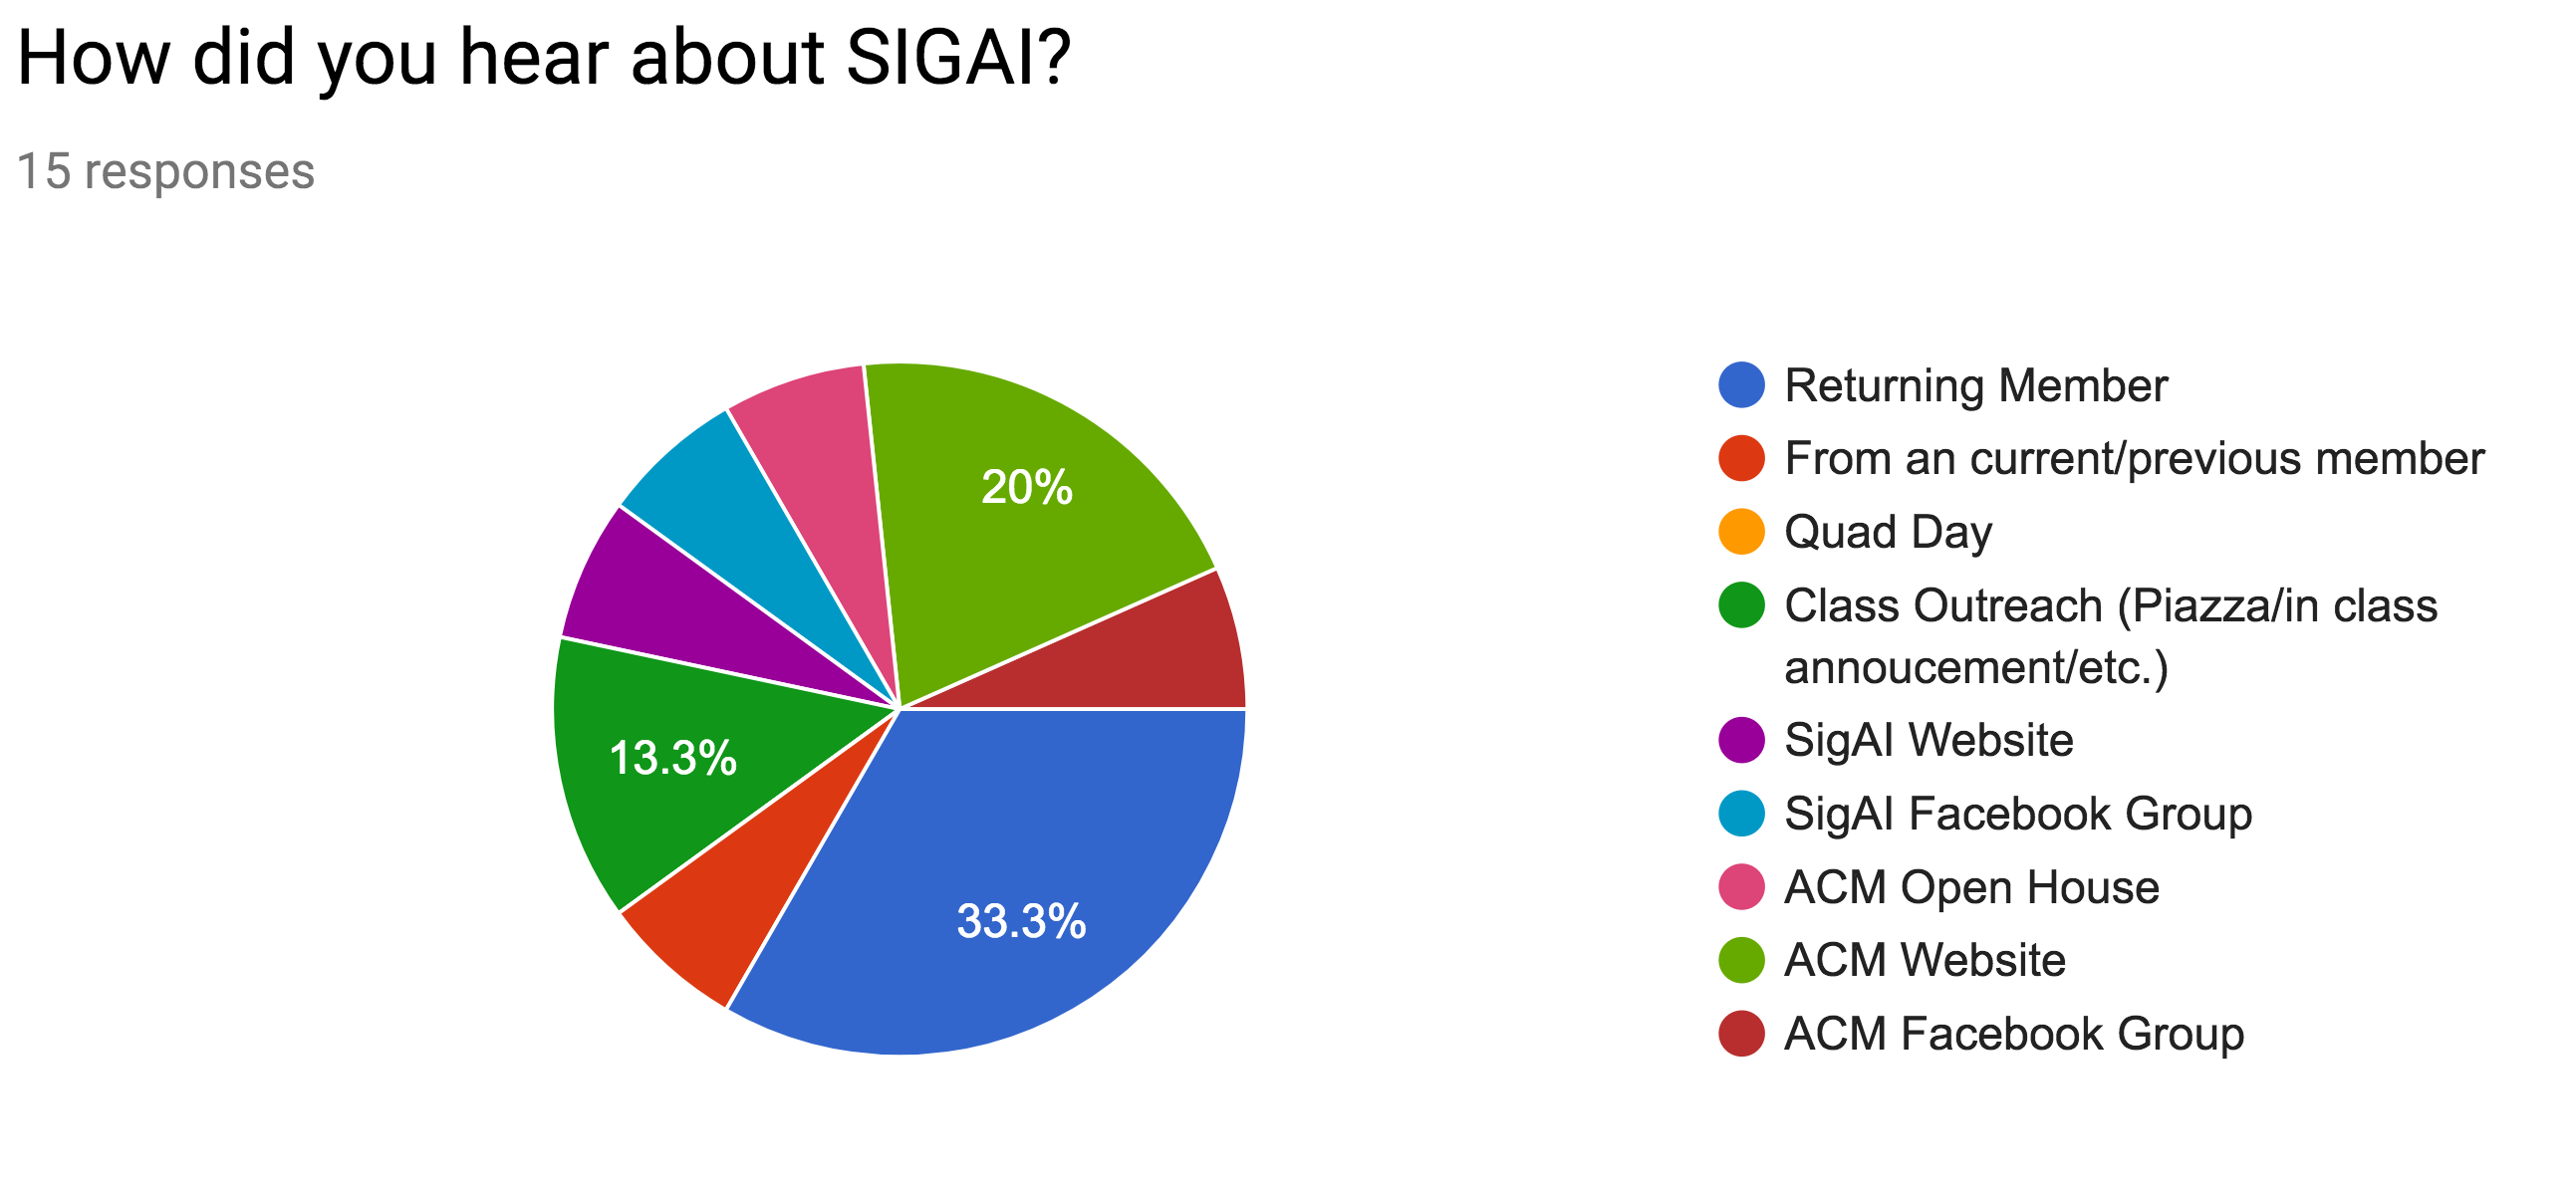
\includegraphics[width=0.8\linewidth]{feedback1.png}
  \end{center}
\end{frame}
\begin{frame}
  \begin{center}
    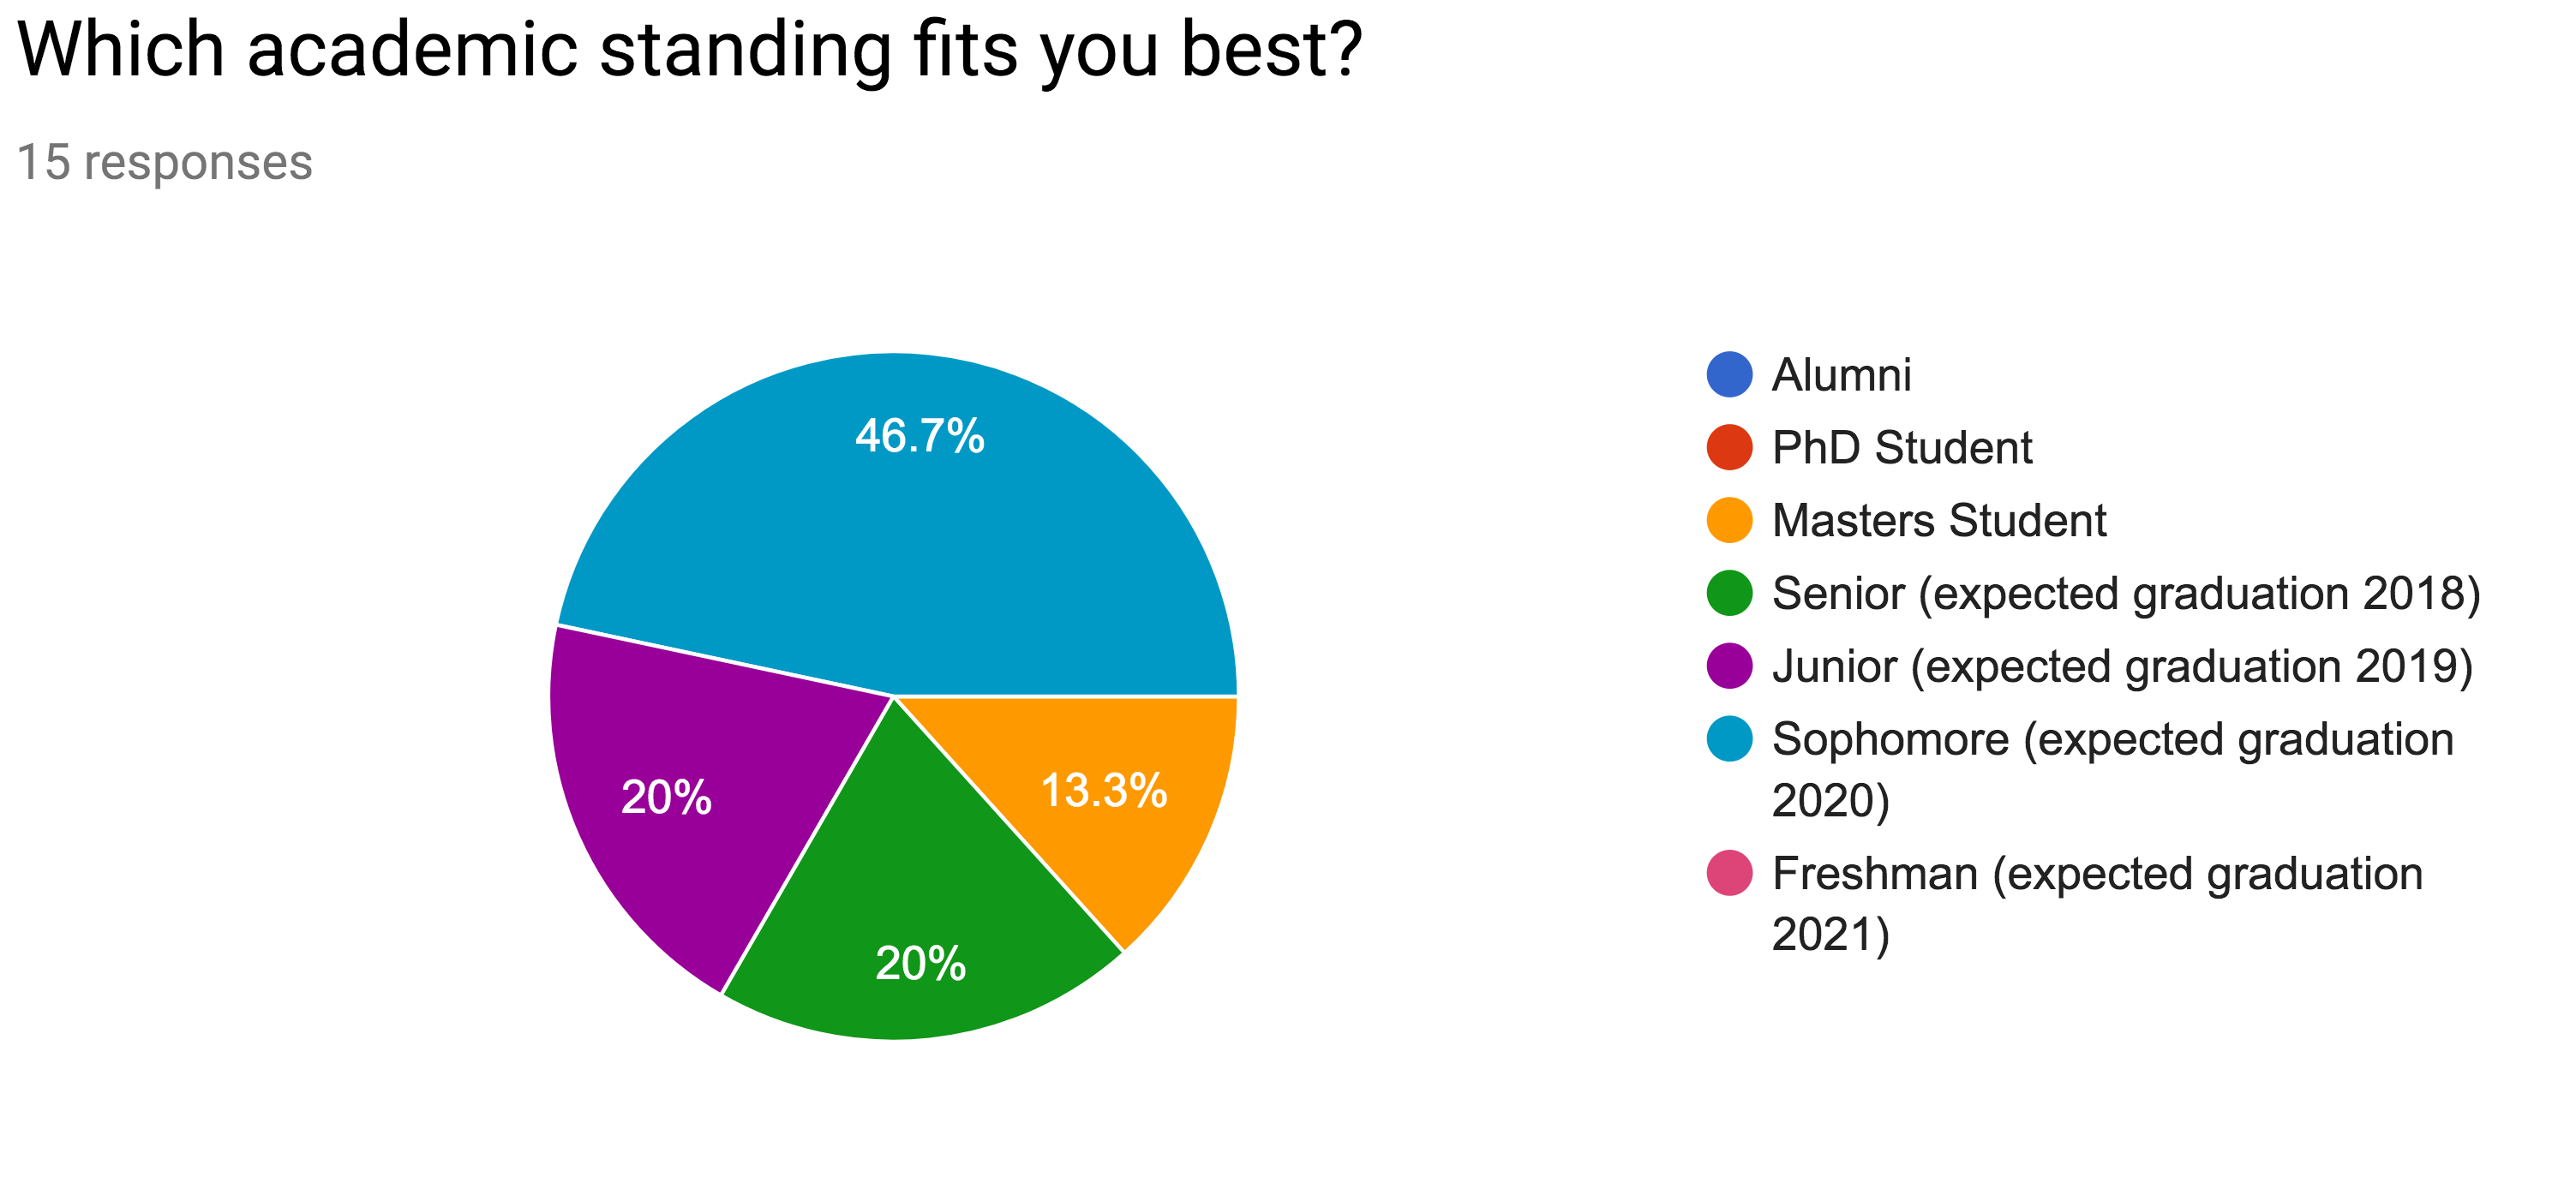
\includegraphics[width=0.8\linewidth]{feedback2.png}
  \end{center}
\end{frame}
\begin{frame}
  \begin{center}
    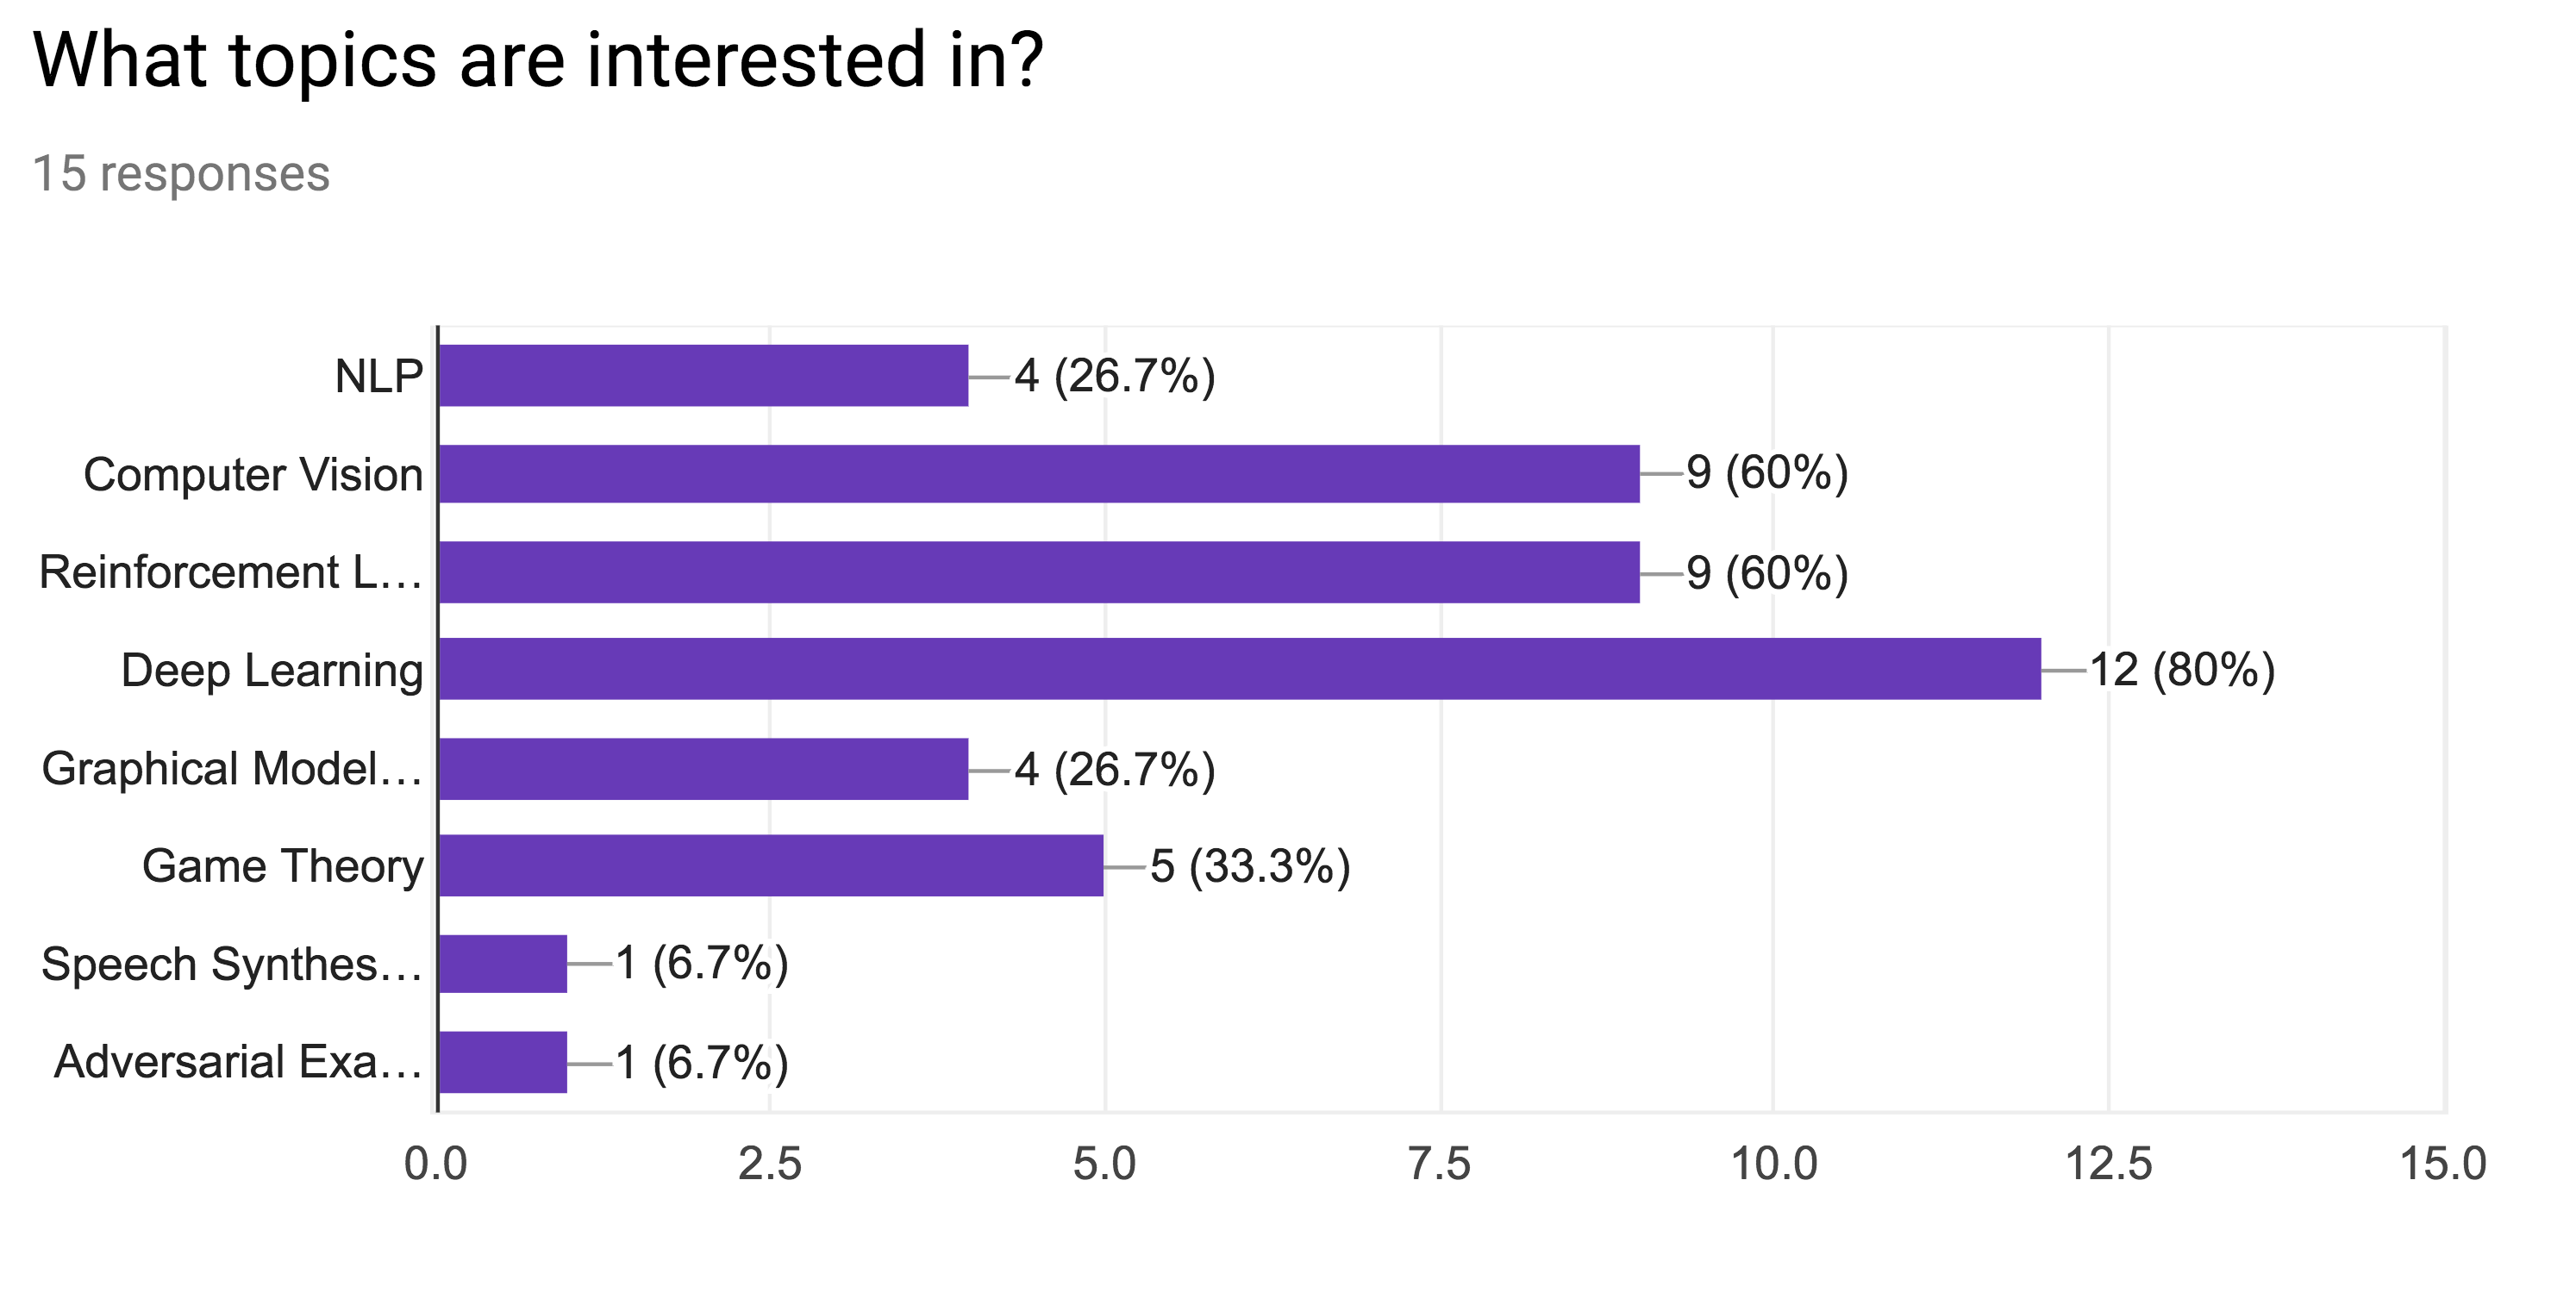
\includegraphics[width=0.8\linewidth]{feedback3.png}
  \end{center}
\end{frame}
\begin{frame}
  \begin{center}
    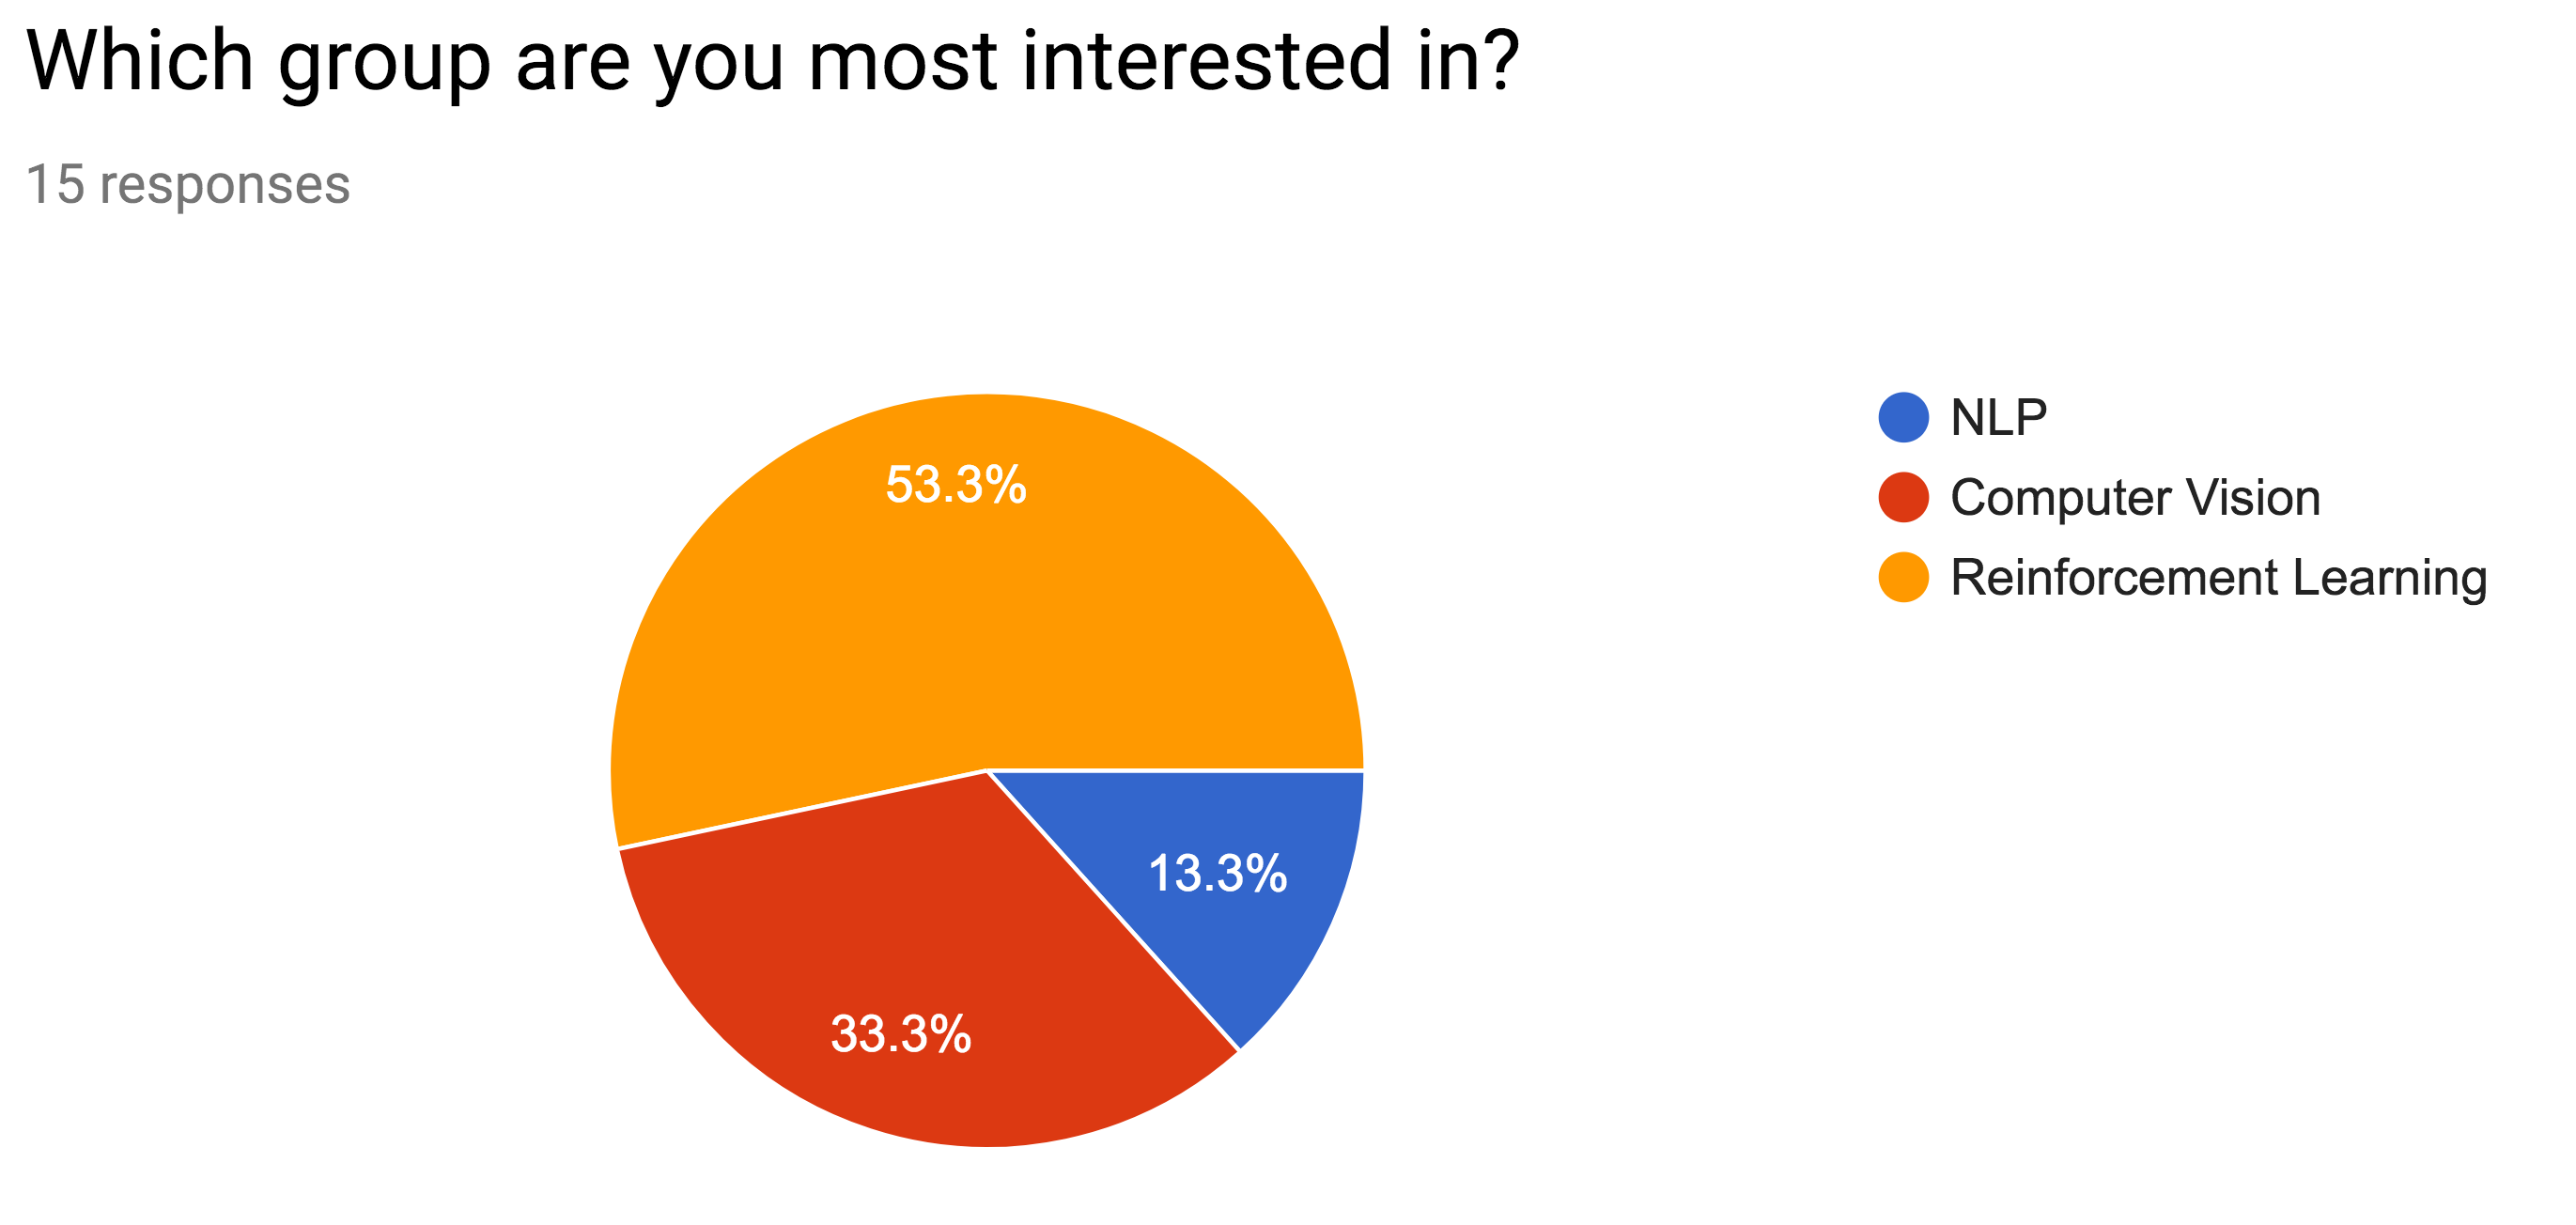
\includegraphics[width=0.8\linewidth]{feedback4.png}
  \end{center}
\end{frame}
\begin{frame}
  \begin{center}
    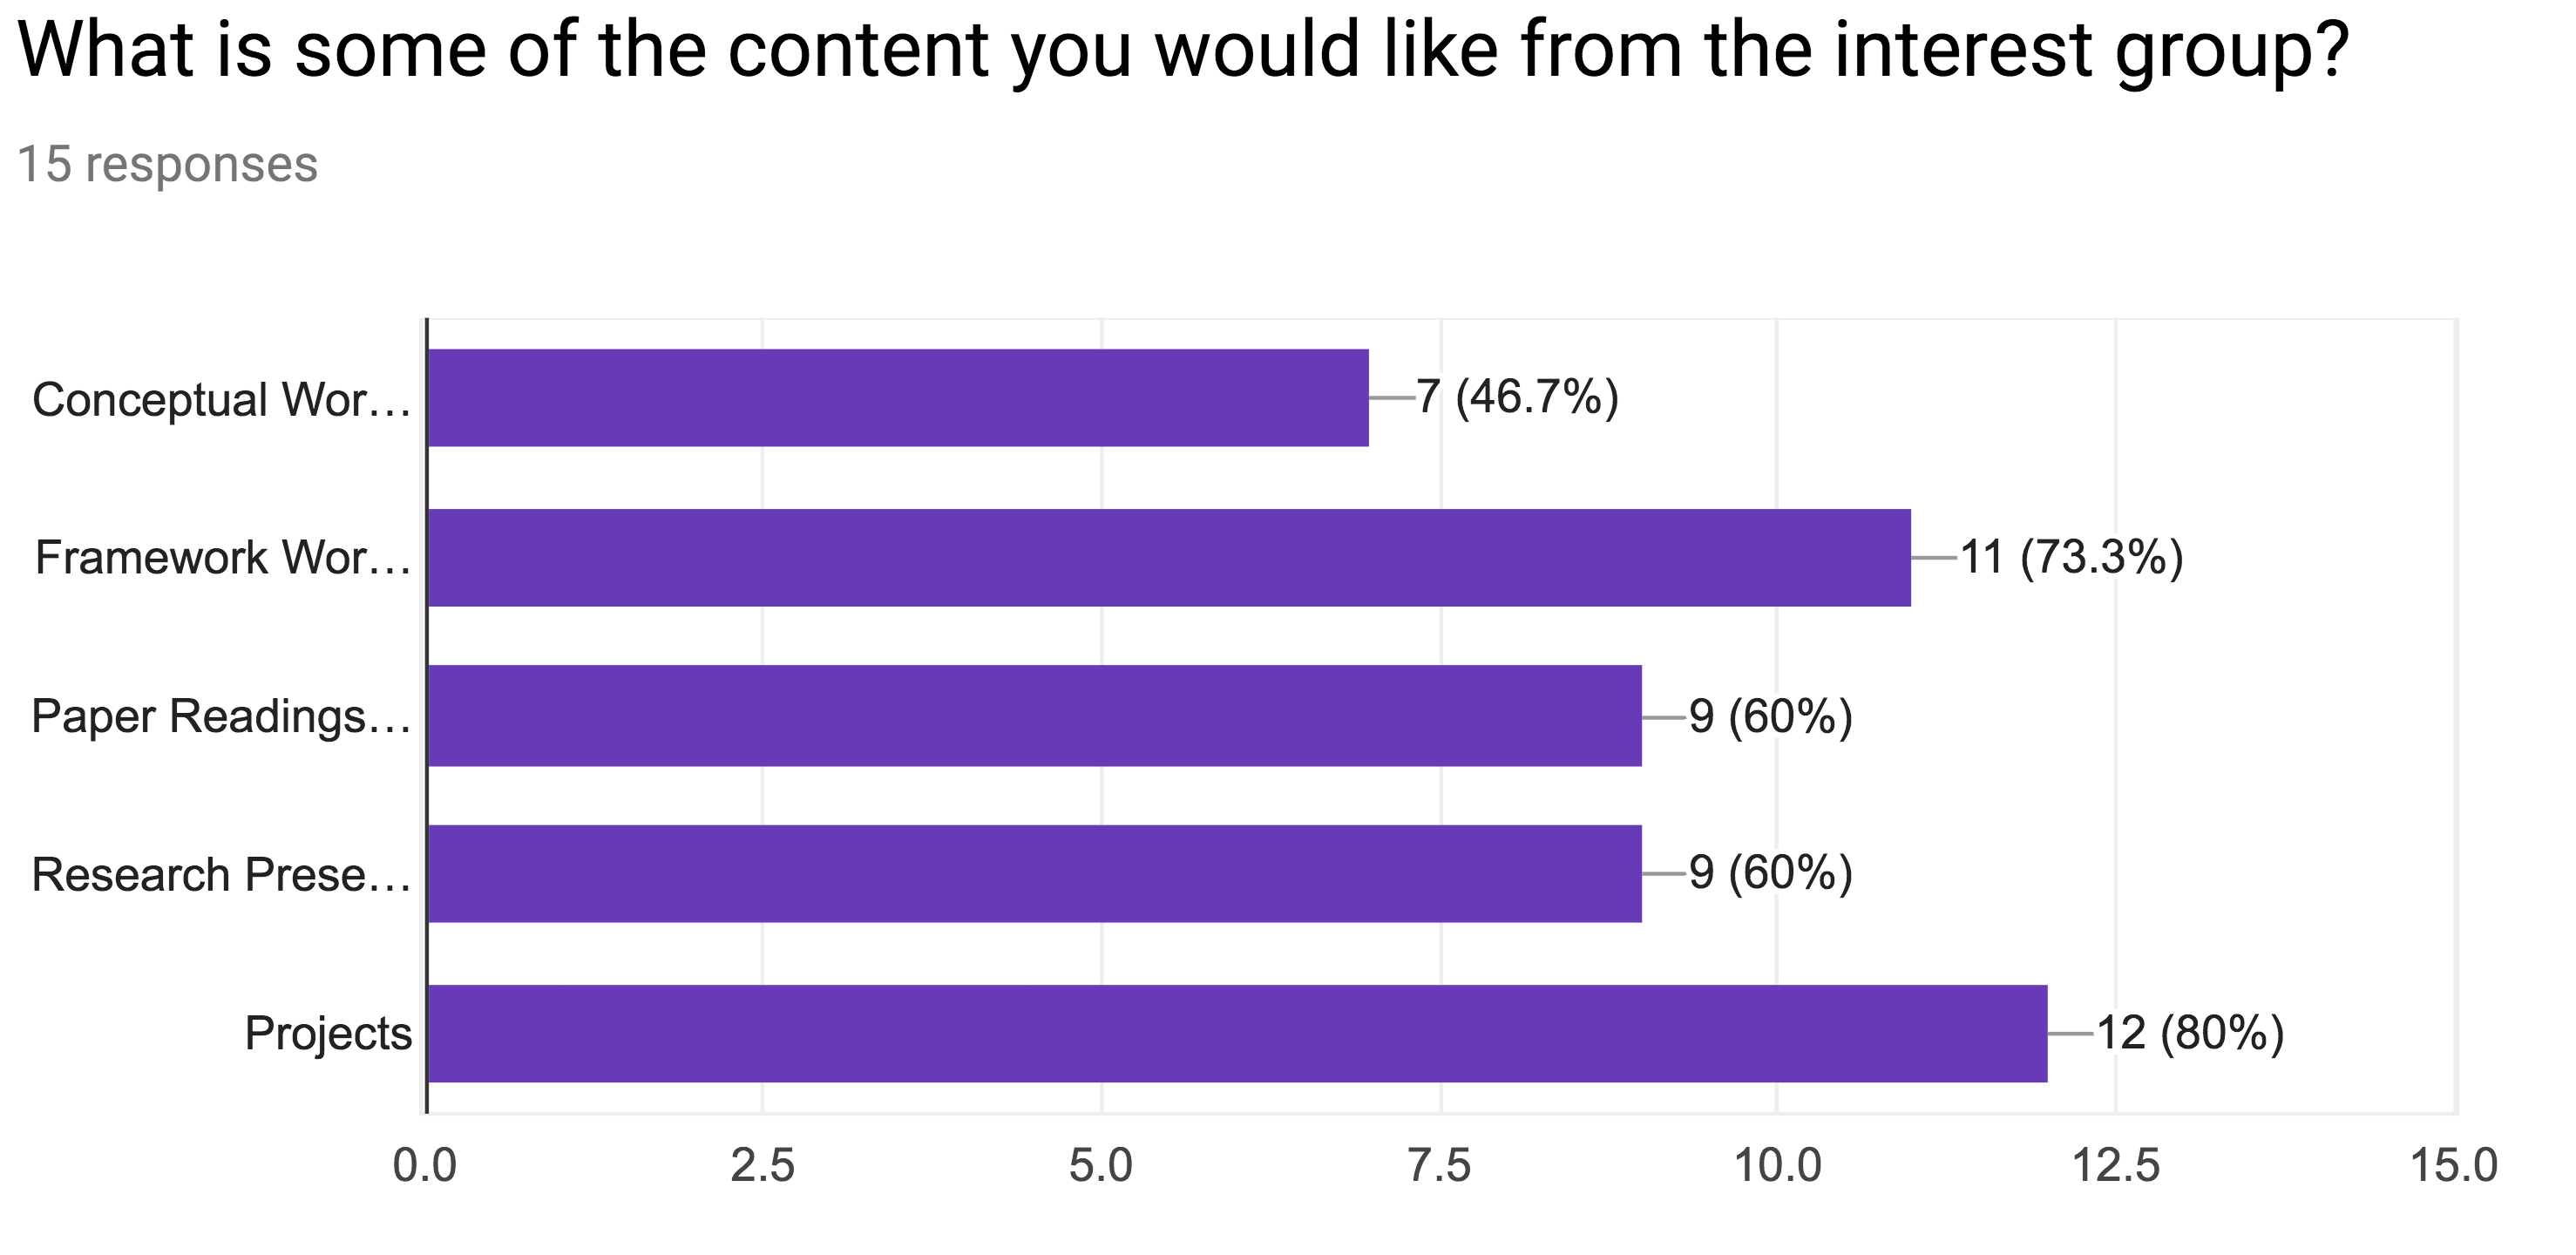
\includegraphics[width=0.8\linewidth]{feedback5.png}
  \end{center}
\end{frame}
\begin{frame}
  \begin{center}
    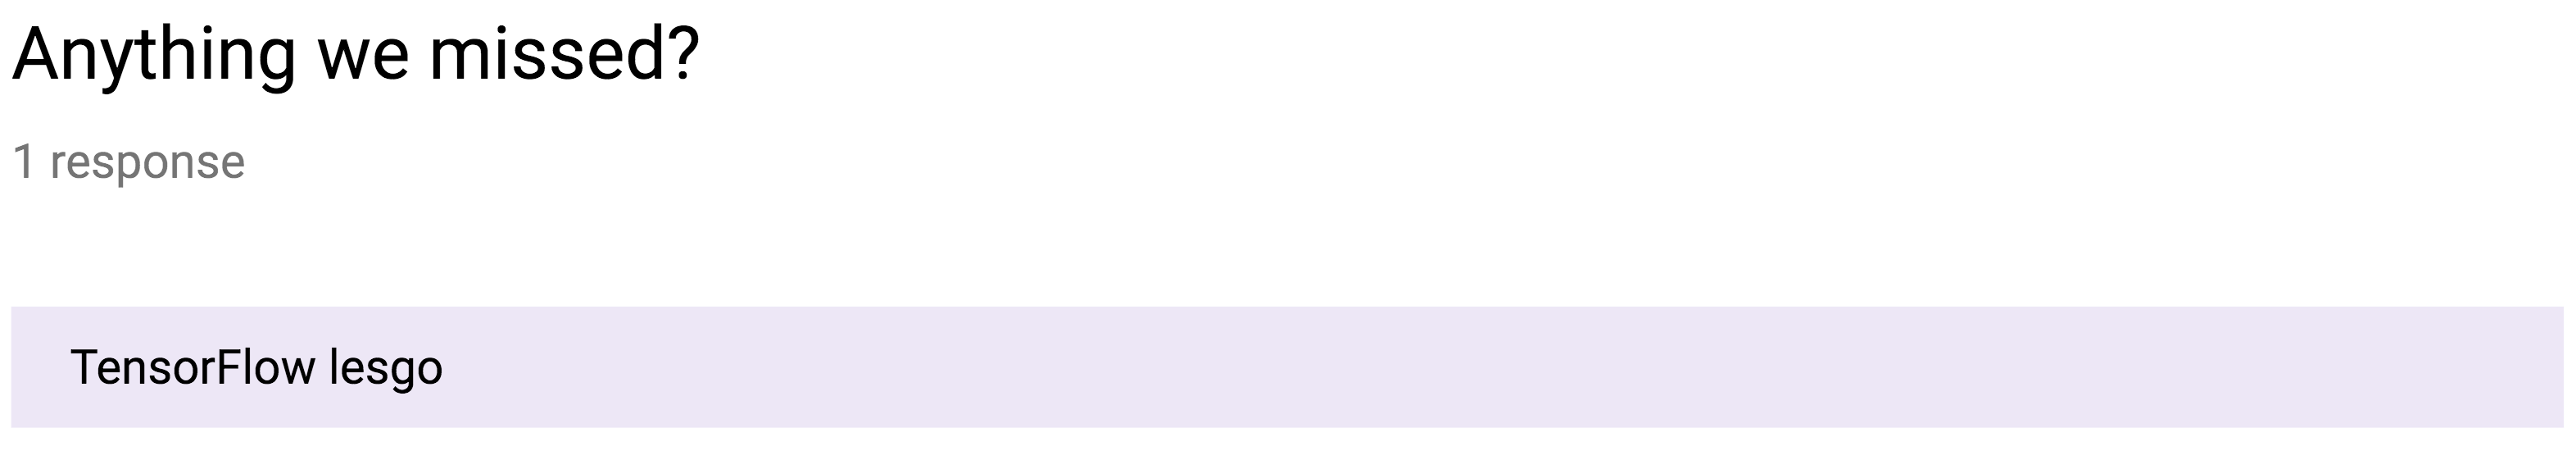
\includegraphics[width=0.8\linewidth]{feedback6.png}
  \end{center}
\end{frame}

\section{Meeting Activities Today}
\begin{frame}
  \frametitle{Vision Group}
  \begin{itemize}
  \item Dominic will go over Single Shot Detectors
  \end{itemize}
\end{frame}

\begin{frame}
  \frametitle{RL Group}
  \begin{itemize}
  \item William Barbour will be giving a presentation about his research and application of Reinforcement Learning.
  \end{itemize}
\end{frame}

\section{Upcoming Events}
\begin{frame}
  \frametitle{Upcoming Events}
  \begin{itemize}
  \item SIGAI might be running a PyTorch Workshop for general ACM members (TBD)
  \item Aim for Spring EOH projects
  \end{itemize}
\end{frame}

\section{Tensorflow Workshop Review}
\begin{frame}
  \frametitle{Tensorflow Workshop Review}
  \begin{itemize}
  \item There was a bug in the workshop slides with LeNet.
  \item GitHub was updated, so make sure you check that.
  \item Akshay will give a small review of main ideas and how to structure Tensorflow Code
  \end{itemize}
\end{frame}


% ----------------------------------------------------------------------------------------
% PRESENTATION SLIDES
% ----------------------------------------------------------------------------------------

\end{document}